\documentclass{ijis}

\usepackage{tikz}
\usetikzlibrary{arrows.meta,positioning,calc,fit,backgrounds}

\definecolor{famML}{HTML}{2A78D6}
\definecolor{famST}{HTML}{EB6834}
\definecolor{famTR}{HTML}{1BAF7A}
\definecolor{inktwo}{HTML}{52514E}
\definecolor{rulegray}{HTML}{C3C2B7}

% Expandable \input, so generated rows can sit directly before \bottomrule inside a tabular.
\makeatletter\newcommand{\inputtable}[1]{\@@input #1 }\makeatother

\title{The Cost of Accuracy in Text Classification: Tradeoffs in Data Representation and Model Design for Classical ML, Neural Network, and Transformer-based Models}
\author{Peter J. Worth Jr.}
\runningauthors{P. J. Worth Jr.}
\hypersetup{pdftitle={The Cost of Accuracy in Text Classification: Tradeoffs in Data Representation and Model Design for Classical ML, Neural Network, and Transformer-based Models}, pdfauthor={Peter J. Worth Jr.}}
\affiliation{Department of Electrical Engineering and Computer Science, Florida Atlantic University, Boca Raton, FL, USA}
\email{pworth2022@fau.edu}
\titlenote{A revised and extended version of \cite{worth2025layercake}, \textit{International Journal of Intelligence Science}, 2025.}
\howtocite{Worth Jr., P.J. (2026) The Cost of Accuracy in Text Classification: Tradeoffs in Data Representation and Model Design for Classical ML, Neural Network, and Transformer-based Models. \textit{International Journal of Intelligence Science}, \textbf{*}, *-*. \url{https://doi.org/10.4236/ijis.2026.*****}}
\license{This work is licensed under the Creative Commons Attribution-NonCommercial International License (CC BY-NC 4.0).\\ \url{http://creativecommons.org/licenses/by-nc/4.0/}}
\ccbadge{
\includegraphics[height=0.52cm]{ijis/cc-by-nc.png}}

\begin{document}

\abstracttext{Fine-tuned transformers are the default choice for text classification, yet the accuracy they add over cheaper alternatives, and the compute they spend to add it, are seldom reported side by side. We measure both across 3,725 training runs of eight classifiers in three families on eight single- and multi-label corpora. The families are linear models (logistic regression, linear SVM, naive Bayes) over sparse, latent-semantic and pooled-embedding features; CNN, LSTM and attention networks over static word embeddings; and seven fine-tuned transformers, from DistilBERT to Llama-3.2-1B and DeepSeek-R1-Distill-Qwen-1.5B. Comparing the best run of each family on each corpus, fine-tuned transformers lead everywhere, but by a mean of only 3.2 Macro-F1 points over the best linear configuration and 6.7 points over the best static-embedding network. Meanwhile, a typical transformer run trains 75 times longer than a typical linear run, and 32 times longer than a typical static-embedding run (127 times its GPU-time). The premium depends on the task. On the four single-label corpora, a linear model within 0.5--2.7 points of the best transformer trains in under 0.5\% of its time; on the four multi-label, many-class corpora, the transformer's 3.7--7.0-point lead over the best linear configuration has no linear substitute. Within the transformer family, the two billion-parameter-scale decoders cost about five times as much to fine-tune as base-size encoders for no consistent gain. Word-class embeddings improve the static-embedding networks (median $+0.8$ points over 129 paired runs), but their token-level analogue has no effect on fine-tuned transformers (median 0.0 over 79 pairs), correcting an earlier report that it degrades them. The strongest linear configurations use frozen, mean-pooled transformer embeddings, whose extraction cost their training time does not include. We release the run-level results and the analysis scripts.}
\keywords{Text Classification, Computational Cost, Fine-Tuning, Transformers, Large Language Models, Word Embeddings, Word-Class Embeddings, Language Representation, Pareto Efficiency, Green AI}

\maketitle

% ============================================================================
\section{Introduction}
% ============================================================================

Text classification is among the most widely deployed tasks in natural language processing: topic routing, spam and abuse filtering, clinical coding, sentiment monitoring and threat triage all reduce to assigning labels to documents. Since BERT \cite{devlin-etal-2019-bert}, the standard recipe has been to fine-tune a pretrained transformer \cite{vaswani,howard2018universal,sun2019fine}, and the models used for that recipe have grown from roughly a hundred million parameters to billions \cite{grattafiori2024llama3,guo2025deepseek}. Benchmarks and surveys of text classification report how much more accurate these models are \cite{minaee2021deep,li2022survey,kowsari2019text}; they rarely report what that accuracy costs to obtain. Calls to report compute alongside accuracy are by now several years old \cite{strubell2019energy,schwartz2020green,dodge2019show,henderson2020towards}, and the energy and dollar cost of large models has been documented at length \cite{patterson2021carbon,luccioni2024power}. What a practitioner choosing a classifier still lacks is a direct answer to two questions about their own task: \emph{how many points of F1 does a fine-tuned transformer add over the cheapest competitive alternative, and how much additional training compute does each of those points require?}

There are good reasons to expect the answer to vary. Linear models over sparse features remain strong text classifiers \cite{joachims1998text,wang2012baselines,joulin-etal-2017-bag}, simple pooled word embeddings are competitive with far more elaborate encoders \cite{shen2018baseline}, and a wide bag-of-words perceptron matches or beats graph-based classifiers on standard benchmarks, although fine-tuned transformers still lead \cite{galke2022bag}. At the same time, fine-tuned small models still outperform prompted generative LLMs on supervised classification, whether the LLMs are used zero-shot or with in-context examples \cite{bucher2024fine,edwards2024language}, so fine-tuning is not going away. A useful study therefore has to place classical, static-embedding and transformer classifiers on a common footing and measure effectiveness and cost on the same runs.

This article does so. We build on Layer Cake, an open benchmarking framework that runs three families of classifiers (linear models, neural networks over static word embeddings, and fine-tuned transformers) over eight single- and multi-label corpora, logging Macro- and Micro-F1, training time and hardware for every run \cite{worth2025layercake}. Here we re-analyse its 3,725 runs as a cost--effectiveness study. We separate the \emph{peak} score a family can reach on a corpus from its \emph{typical} score across configurations. We test family differences with paired non-parametric tests across corpora \cite{demsar2006statistical}, express cost both as wall-clock training time and as accelerator-time, and trace, for each corpus, the Pareto frontier of score against training time and the cheapest run within a given tolerance of the best. We also ask two narrower questions the earlier study raised but did not settle: whether larger transformers are worth their cost, and whether supervised class embeddings help the models they are attached to.

Five findings stand out.
\begin{enumerate}
\setlength\itemsep{1pt}
\item \textbf{The transformer premium is real but small on average.} At peak, fine-tuned transformers beat the best linear configuration on all eight corpora, but by a mean of 3.2 Macro-F1 points (range 0.1--7.0), and the best static-embedding network by 6.7 points (0.4--16.8). A typical transformer run takes 75 times as long to train as a typical linear run and 32 times as long as a typical static-embedding run (127 times the GPU-time; geometric means).
\item \textbf{The premium depends on the task.} On the four single-label corpora the best linear configuration trails by 0.1--2.3 points, and a linear run within 0.5--2.7 points of the best transformer costs 0.2--0.5\% of its training time. On the four multi-label corpora, which have 23--115 classes, the transformer's lead of 3.7--7.0 points cannot be obtained without a transformer.
\item \textbf{Linear models over frozen transformer embeddings beat static-embedding networks.} The best linear configuration outperforms the best CNN, LSTM or attention network over static word vectors on every corpus (mean $+3.5$ Macro-F1), and no static-embedding run lies on any Macro-F1 Pareto frontier. On six of the eight corpora the winning linear configuration uses mean-pooled embeddings from a frozen transformer, whose one-off extraction cost is not included in its training time.
\item \textbf{Larger transformers are not worth their cost here.} DeepSeek-R1-Distill-Qwen-1.5B has the best average rank among the seven fine-tuned models but takes 6.6 times as long to train as BERT; Llama-3.2-1B ranks sixth of seven at 5.1 times. Against the best base-size encoder on each corpus, the better of the two large models changes Macro-F1 by a median of $-0.4$ points at 4.9 times the training time.
\item \textbf{Class embeddings help static networks, not transformers.} Appending word-class embeddings (WCEs) \cite{moreo2021} to static word vectors raises Macro-F1 in 80 of 129 paired runs (median $+0.8$, $p = 1.5\times10^{-6}$). Fusing the token-level analogue (TCEs) with a fine-tuned transformer changes nothing (median 0.0 across 79 pairs, $p = 0.66$).
\end{enumerate}

\paragraph{Contributions.}
\begin{enumerate}
\setlength\itemsep{1pt}
\item[(i)] A controlled comparison of eight classifiers in three families on eight corpora in which effectiveness and training cost are measured on the same runs. It comes with a reporting protocol (peak and typical scores, paired tests, accelerator-time, Pareto frontiers and tolerance tables) that keeps the two quantities apart.
\item[(ii)] Evidence that the transformer premium is concentrated in multi-label, many-class tasks, with the cheapest near-equivalent run identified for every corpus.
\item[(iii)] Evidence that linear models over pooled frozen embeddings dominate static-embedding networks and populate most of the low-cost frontier, with an explicit statement of what that comparison leaves out.
\item[(iv)] Paired analyses showing that billion-parameter-scale decoders do not repay their cost over base encoders on these tasks, and that class embeddings help static but not contextual models.
\item[(v)] The run-level results and every analysis script, so that each number and figure can be regenerated.
\end{enumerate}

\paragraph{Relation to the earlier version.} This article revises and extends \cite{worth2025layercake}. The experimental runs are the same, but the analysis is new and is computed from the run-level records, which reproduce every summary statistic published earlier. We replace pooled averages over unequal numbers of configurations with per-corpus peak and typical comparisons. We add significance tests, accelerator-time, Pareto, tolerance, model-size and paired class-embedding analyses. Re-deriving the earlier paper's results led to three substantive corrections:
\begin{itemize}
\setlength\itemsep{1pt}
\item Its headline comparison with classical models (a 12.73\% Macro-F1 advantage for transformers) contrasted the best transformer with the \emph{average} classical configuration. Against the best classical configuration the advantage is 4.2\% (3.2 points), and we report both.
\item Its report that token-class embeddings degraded transformer performance is not borne out by the logged runs; they have no measurable effect.
\item Its descriptions of the hardware, language-model checkpoints and datasets contained errors, which are corrected here from the run logs and the model configurations.
\end{itemize}

The rest of the article is organised as follows. Section~\ref{sec:background} reviews related work. Section~\ref{sec:setup} describes the framework, data, models, hardware and analysis protocol. Section~\ref{sec:results} reports results, Section~\ref{sec:discussion} discusses practical implications and limitations, and Section~\ref{sec:conclusion} concludes.

% ============================================================================
\section{Background and Related Work}\label{sec:background}
% ============================================================================

\subsection{From sparse vectors to contextual representations}

Early statistical text classifiers represented a document as a sparse vector over the vocabulary, weighted by term frequency and inverse document frequency \cite{sparckjones1972statistical,salton1971smart}. Because such vectors have tens of thousands of dimensions, they were often compressed, most commonly by latent semantic analysis (LSA), a truncated singular value decomposition of the term--document matrix \cite{deerwester}. Dense learned word vectors appeared with neural language models \cite{bengio2003neural,collobert2011natural} and became ubiquitous with word2vec \cite{mikolov,mikolov2013distributed}, GloVe \cite{pennington} and fastText \cite{articleboja,mikolov2018advances}. All of these rest on the distributional hypothesis, that words occurring in similar contexts have similar meanings \cite{harris,firth}, and all assign one vector per word type, so they cannot represent the sense a word takes in context \cite{worth}.

Contextual representations remove that limitation. ELMo derived token vectors from a bidirectional LSTM language model \cite{peters2018deep}. The transformer \cite{vaswani}, building on attention for sequence transduction \cite{bahdanau2016neuralmachinetranslationjointly}, made it practical to pretrain deep contextual encoders such as BERT \cite{devlin-etal-2019-bert}, RoBERTa \cite{liu2019roberta} and XLNet \cite{yang2019xlnet}, and decoder-only models such as GPT-2 \cite{radford2019language}. Distillation produces smaller variants such as DistilBERT \cite{hinton2015distilling,sanh2020distilbert}. Current open decoder models, including the Llama~3 family \cite{grattafiori2024llama3} and models distilled from DeepSeek-R1 into Qwen2.5 bases \cite{guo2025deepseek,yang2024qwen25}, are larger again. All of these models operate on subword vocabularies produced by WordPiece \cite{schuster,wu}, byte-pair encoding \cite{gage1994,sennrich-etal-2016-neural} or SentencePiece \cite{kudo2018sentencepiece}. The size of that vocabulary fixes the size of the model's input embedding matrix, a point that matters for the cost comparisons below.

\subsection{Classifiers for text}

Linear classifiers over sparse features (naive Bayes \cite{mccallum1998comparison}, support vector machines \cite{joachims1998text} and regularised logistic regression \cite{genkin01082007}) defined the state of the art for two decades \cite{sebastiani2002machine}. Neural classifiers over static embeddings followed: convolutional networks \cite{yoon2014convolutional,zhang2015character}, recurrent networks built on LSTM units \cite{hochreiterlong}, and attention-based recurrent models \cite{liuguo2019bidirectional}. Fine-tuning a pretrained language model end to end \cite{howard2018universal,devlin-etal-2019-bert,sun2019fine} then became standard. Surveys trace this progression \cite{kowsari2019text,minaee2021deep,li2022survey,qiu2020pre}, and recent studies revisit text classification in the age of large language models \cite{trust2024study} and compare fine-tuned small models with prompted LLMs \cite{bucher2024fine,edwards2024language}. These studies compare effectiveness; they do not report the training cost of each approach on the same runs.

\subsection{Strong baselines and the cost of accuracy}

A recurring finding is that simple models are hard to beat:
\begin{itemize}
\setlength\itemsep{1pt}
\item Wang and Manning showed that naive-Bayes-weighted linear models are strong baselines for topic and sentiment classification \cite{wang2012baselines}.
\item fastText showed that a linear model over averaged word and n-gram embeddings is often on par with deep classifiers in accuracy while training orders of magnitude faster \cite{joulin-etal-2017-bag}.
\item SWEM showed that pooled word embeddings rival recurrent and convolutional encoders \cite{shen2018baseline}.
\item Galke and Scherp showed that a wide multilayer perceptron over bag-of-words features matches or outperforms graph-based classifiers, while fine-tuned BERT and DistilBERT remain ahead \cite{galke2022bag}.
\end{itemize}

Separately, a literature on the cost of NLP has made three arguments: efficiency should be reported as a first-class result \cite{strubell2019energy,schwartz2020green,henderson2020towards}; results should be reported as a function of the computational budget spent to obtain them \cite{dodge2019show}; and task-specific models are far cheaper to run than general-purpose ones \cite{luccioni2024power}. Efficiency methods for transformers have been surveyed in depth \cite{treviso2023efficient}. Among them, parameter-efficient fine-tuning reduces the number of trainable weights through adapters \cite{pmlr-v97-houlsby19a}, prefix tuning \cite{li2021prefixtuningoptimizingcontinuousprompts}, low-rank adaptation \cite{hu2021loralowrankadaptationlarge} and its quantised and adaptive variants \cite{dettmers2023qloraefficientfinetuningquantized,zhang2023adaloraadaptivebudgetallocation}, reviewed in \cite{articleding}. Our study sits between these literatures: we evaluate full fine-tuning, the most expensive common practice, against the strong cheap baselines that the first literature recommends, and we report cost in the way the second recommends.

\subsection{Supervised class embeddings}

Word-class embeddings (WCEs) represent each vocabulary term by its correlation with each class in the training set, computed from the co-occurrence of terms and labels in the training documents \cite{moreo2021}; the code base supports several such supervised functions, including a normalised dot product, positive pointwise mutual information, information gain and $\chi^2$. Concatenated to pretrained word vectors, they add class-specific evidence that general-purpose embeddings lack. Moreo et al.\ report consistent gains when WCEs are added to four neural architectures for topic classification \cite{moreo2021}, and Layer Cake inherits its static-embedding neural module from that work. Whether the same information helps a fine-tuned transformer, whose representations are themselves shaped by the labels during fine-tuning, has not been tested on matched runs; Section~\ref{sec:classemb} provides that test.

% ============================================================================
\section{Experimental Framework}\label{sec:setup}
% ============================================================================

\subsection{Overview}

Layer Cake runs three modules that share datasets, splits and logging but differ in how text is represented and which hardware they use (\figref{fig:framework}). The classical module trains scikit-learn classifiers \cite{pedregosa2011scikit}; the static-embedding module, extended from the code of \cite{moreo2021}, trains PyTorch networks \cite{paszke2019pytorch} over pretrained word vectors; and the transformer module fine-tunes Hugging Face models \cite{wolf2020transformers}. Every run writes one record per metric with the corpus, classifier, language model, representation, hyperparameters, training time, operating system, CPU, GPU and memory. All code is available at \url{https://github.com/pworth1971/layer-cake}.

\begin{figure}[t]
\centering
\resizebox{\linewidth}{!}{%
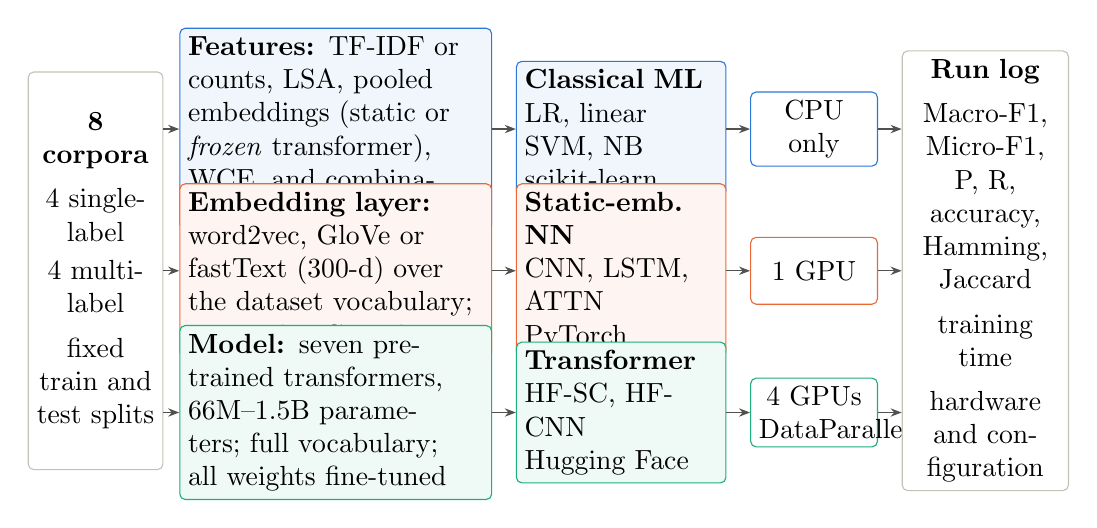
\begin{tikzpicture}[
    font=\figfont, >={Stealth[length=4pt]}, node distance=0.3cm,
    lane/.style={draw=#1, fill=#1!7, rounded corners=2pt, align=left, inner sep=3pt, minimum height=1.45cm},
    side/.style={draw=rulegray, fill=white, rounded corners=2pt, align=center, inner sep=3pt},
    hw/.style={draw=#1, fill=white, rounded corners=2pt, align=center, inner sep=3pt, text width=1.4cm, minimum height=0.85cm},
    arr/.style={->, draw=inktwo, line width=0.5pt}]
  \node[lane=famML, text width=3.75cm] (r1) at (3.85,0) {\textbf{Features:} TF-IDF or counts, LSA, pooled embeddings (static or \emph{frozen} transformer), WCE, and combinations};
  \node[lane=famST, text width=3.75cm] (r2) at (3.85,-1.8) {\textbf{Embedding layer:} word2vec, GloVe or fastText (300-d) over the dataset vocabulary; optional WCE columns};
  \node[lane=famTR, text width=3.75cm] (r3) at (3.85,-3.6) {\textbf{Model:} seven pretrained transformers, 66M--1.5B parameters; full vocabulary; all weights fine-tuned};
  \node[lane=famML, text width=2.45cm, right=of r1] (c1) {\textbf{Classical ML}\\ LR, linear SVM, NB\\ scikit-learn};
  \node[lane=famST, text width=2.45cm, right=of r2] (c2) {\textbf{Static-emb.\ NN}\\ CNN, LSTM, ATTN\\ PyTorch};
  \node[lane=famTR, text width=2.45cm, right=of r3] (c3) {\textbf{Transformer}\\ HF-SC, HF-CNN\\ Hugging Face};
  \node[hw=famML, right=of c1] (h1) {CPU only};
  \node[hw=famST, right=of c2] (h2) {1 GPU};
  \node[hw=famTR, right=of c3] (h3) {4 GPUs\\ DataParallel};
  \node[side, text width=1.5cm, minimum height=5.05cm] (ds) at (0.8,-1.8) {\textbf{8 corpora}\\[4pt] 4 single-label\\[2pt] 4 multi-label\\[4pt] fixed train and test splits};
  \node[side, text width=1.9cm, minimum height=5.05cm, right=of h2] (log) {\textbf{Run log}\\[4pt] Macro-F1, Micro-F1, P, R, accuracy, Hamming, Jaccard\\[4pt] training time\\[4pt] hardware and configuration};
  \foreach \i in {1,2,3} {
    \draw[arr] (ds.east |- r\i.west) -- (r\i.west);
    \draw[arr] (r\i) -- (c\i);
    \draw[arr] (c\i) -- (h\i);
    \draw[arr] (h\i.east) -- (log.west |- h\i.east);
  }
\end{tikzpicture}}
\caption{The three Layer Cake modules. Each corpus is processed by all three; colours mark the classifier family throughout the article. The classical module can consume embeddings from the same static and transformer language models used by the other two modules, but only as frozen, pooled features.}
\label{fig:framework}
\end{figure}

\subsection{Datasets}

\tabref{tab:datasets} lists the eight corpora, grouped by task type. The single-label corpora are:
\begin{itemize}
\setlength\itemsep{1pt}
\item BBC News: the 1,490 labelled articles distributed for the Kaggle BBC News classification task, drawn from the corpus of \cite{greene};
\item 20~Newsgroups, with its standard by-date split \cite{LANG1995331};
\item the IMDB sentiment corpus, with its 25,000/25,000 split \cite{maas};
\item ArXiv-10: 100,000 abstracts in ten subject categories, released with Protoformer \cite{farhangi}.
\end{itemize}
The multi-label corpora are:
\begin{itemize}
\setlength\itemsep{1pt}
\item Reuters-21578, with the ModApt\'e split \cite{lewis1987reuters};
\item OHSUMED medical abstracts labelled with 23 MeSH disease categories \cite{hersh1994ohsumed,joachims1998text};
\item a 58-category corpus of arXiv abstracts built from the public arXiv metadata \cite{clement2019use};
\item RCV1-v2, with the LYRL2004 split, in which only 23,149 of 804,414 documents are used for training \cite{lewis2004}. RCV1-v2 defines 103 topic categories, of which the 101 that occur in this split are used.
\end{itemize}
The classical module trains on the full training split. The neural modules hold out part of it for validation and early stopping on validation Macro-F1: 20\% in the static-embedding module and 17.5\% in the transformer module (exact sizes in Appendix~\ref{app:splits}). Test sets are identical across modules.

\begin{table}[t]
\centering
\footnotesize
\caption{Corpora. Classes are those occurring in the split used. Train and test sizes are those of the classical module; the neural modules hold out part of the training split for validation.}
\label{tab:datasets}
\begin{tabular}{@{}llrrrr@{}}
\toprule
\textbf{Corpus} & \textbf{Domain} & \textbf{Classes} & \textbf{Documents} & \textbf{Train} & \textbf{Test} \\
\midrule
\multicolumn{6}{@{}l}{\textit{Single-label}} \\
\inputtable{tables/tab_datasets.tex}
\bottomrule
\end{tabular}
\end{table}

\subsection{Representations and language models}\label{sec:representations}

\paragraph{Language models.} \tabref{tab:lms} lists the ten pretrained models. The three static models supply one 300-dimensional vector per word type. The fastText vectors used are the word-level Common Crawl vectors of \cite{mikolov2018advances}, without subword information, so out-of-vocabulary words are treated the same way for all three static models. The seven transformer models range from 66M to about 1.5B parameters and use three tokenizer families.

\begin{table}[t]
\centering
\scriptsize
\begin{fullwidth}
\caption{Pretrained language models. For static models the vocabulary column gives the number of word vectors; for transformers it gives the tokenizer vocabulary, which fixes the number of rows in the input embedding matrix. Parameter counts are approximate. Training data are as reported by the model authors.}
\label{tab:lms}
\renewcommand{\arraystretch}{1.15}
\begin{tabularx}{\linewidth}{@{}l>{\raggedright}X l r r >{\raggedright\arraybackslash}X@{}}
\toprule
\textbf{Model} & \textbf{Objective} & \textbf{Tokenizer} & \textbf{Vocab.} & \textbf{Dim.} & \textbf{Pretraining data} \\
\midrule
GloVe \cite{pennington} & co-occurrence factorisation & word & 2.2M & 300 & Common Crawl, 840B tokens \\
word2vec \cite{mikolov,mikolov2013distributed} & negative sampling & word & 3.0M & 300 & Google News, $\sim$100B words \\
fastText \cite{mikolov2018advances} & CBOW, position weights & word & 2.0M & 300 & Common Crawl, 600B tokens \\
\midrule
BERT (110M) \cite{devlin-etal-2019-bert} & masked LM + NSP & WordPiece & 30,522$^{a}$ & 768 & BooksCorpus, Wikipedia \\
DistilBERT (66M) \cite{sanh2020distilbert} & distillation from BERT & WordPiece & 28,996 / 30,522$^{b}$ & 768 & as BERT \\
RoBERTa (125M) \cite{liu2019roberta} & masked LM & byte-level BPE & 50,265 & 768 & 160\,GB of books, web, news \\
XLNet (117M) \cite{yang2019xlnet} & permutation LM & SentencePiece & 32,000 & 768 & books, Wikipedia, web \\
GPT-2 (124M) \cite{radford2019language} & next-token prediction & byte-level BPE & 50,257 & 768 & WebText \\
Llama-3.2 (1.23B) \cite{grattafiori2024llama3,llama32modelcard} & next-token + distillation & BPE (tiktoken) & 128,256 & 2,048 & public data, up to 9T tokens \\
DeepSeek-R1-Distill (1.5B) \cite{guo2025deepseek} & SFT on 800k R1-curated samples & byte-level BPE & 151,936 & 1,536 & Qwen2.5-Math-1.5B base \cite{yang2024qwen25} \\
\bottomrule
\multicolumn{6}{@{}>{\raggedright\arraybackslash}p{\linewidth}@{}}{\rule{0pt}{9pt}Checkpoints: \texttt{glove.840B.300d}, \texttt{GoogleNews-vectors-negative300}, \texttt{crawl-300d-2M}, \texttt{bert-base-uncased}, \texttt{distilbert-base-\{cased,uncased\}}, \texttt{roberta-base}, \texttt{xlnet-base-cased}, \texttt{gpt2}, \texttt{meta-llama/Llama-3.2-1B}, \texttt{deepseek-ai/DeepSeek-R1-Distill-Qwen-1.5B}. $^{a}$Fine-tuned runs use the uncased model, as recorded by the vocabulary size in the run log. $^{b}$Both variants appear in the fine-tuned runs.}
\end{tabularx}
\end{fullwidth}
\end{table}

\paragraph{Preprocessing.} For the static word models, text is lower-cased and stripped of punctuation and stop words. For transformer models, raw text is passed to each model's own tokenizer.

\paragraph{Feature sets for the classical module.} We use the following notation:
\begin{itemize}
\setlength\itemsep{1pt}
\item $\mathbf{x}_d$: the TF-IDF vector of document $d$ (sublinear term frequency, minimum document frequency 5, as in the code base inherited from \cite{moreo2021});
\item $E_M$: the matrix of embeddings that language model $M$ assigns to the vocabulary;
\item $\bar{\mathbf{e}}^{M}_d$: the pooled embedding of $d$. For static models it is the mean (or TF-IDF-weighted mean) of the document's word vectors; for transformers it is the mean of the frozen model's final-layer hidden states over the padded input sequence;
\item $W$: the WCE matrix computed from the training split \cite{moreo2021};
\item $\oplus$: concatenation;
\item $\Pi_{M+\mathrm{WCE}}(d) = \mathbf{x}_d\,[E_M \oplus W]$: the projection of the TF-IDF vector onto the WCE-extended embedding space.
\end{itemize}
The ten feature sets (\emph{representation forms}) are defined in \tabref{tab:forms}. All embeddings are frozen; only the linear classifier is trained.

\begin{table}[t]
\centering
\footnotesize
\caption{Feature sets (representation forms) used by the classical module.}
\label{tab:forms}
\begin{tabular}{@{}lll@{}}
\toprule
\textbf{Name} & \textbf{Features} & \textbf{Dimension} \\
\midrule
vmode & $\mathbf{x}_d$ (TF-IDF or raw counts) & $|V_D|$ \\
lsa & truncated SVD of $\mathbf{x}_d$ & $d_M$ \\
solo & $\bar{\mathbf{e}}^{M}_d$ & $d_M$ \\
dot & $\mathbf{x}_d E_M$ & $d_M$ \\
cat-doc & $\mathbf{x}_d \oplus \bar{\mathbf{e}}^{M}_d$ & $|V_D| + d_M$ \\
\midrule
lsa-wce & $\mathrm{SVD}(\mathbf{x}_d) \oplus \Pi_{M+\mathrm{WCE}}(d)$ & $2d_M + |\mathcal{C}|$ \\
solo-wce & $\bar{\mathbf{e}}^{M}_d \oplus \Pi_{M+\mathrm{WCE}}(d)$ & $2d_M + |\mathcal{C}|$ \\
dot-wce & $\Pi_{M+\mathrm{WCE}}(d)$ & $d_M + |\mathcal{C}|$ \\
cat-wce & $\mathbf{x}_d \oplus \Pi_{M+\mathrm{WCE}}(d)$ & $|V_D| + d_M + |\mathcal{C}|$ \\
cat-doc-wce & $\mathbf{x}_d \oplus \bar{\mathbf{e}}^{M}_d \oplus \Pi_{M+\mathrm{WCE}}(d)$ & $|V_D| + 2d_M + |\mathcal{C}|$ \\
\bottomrule
\end{tabular}
\end{table}

\subsection{Classifiers}

\paragraph{Classical module.} Logistic regression (LR), linear SVM and multinomial naive Bayes (NB) from scikit-learn, with default hyperparameters, wrapped one-vs-rest for multi-label corpora. NB requires non-negative inputs, so it is run only on count and TF-IDF features. Each classifier is run with every compatible combination of feature set, language model and pooling, which yields 171--244 configurations per corpus for LR and the SVM and 18--38 for NB.

\paragraph{Static-embedding module.} CNN \cite{yoon2014convolutional}, LSTM \cite{hochreiterlong} and attention (ATTN) \cite{liuguo2019bidirectional} classifiers, each with GloVe, word2vec and fastText inputs. The pretrained vectors are either frozen or fine-tuned, with and without WCEs, over a small grid of channel or hidden sizes (4--24 runs per classifier and corpus). The embedding layer contains only the words of the corpus vocabulary, plus unknown and padding tokens. WCEs (information gain, z-scored) are appended as extra columns (\figref{fig:embedding}(a)). Single-label corpora use cross-entropy loss and multi-label corpora binary cross-entropy with logits.

\paragraph{Transformer module.} Each of the seven models is fine-tuned in full with two heads: the Hugging Face sequence-classification head (HF-SC) and a convolutional head over the final hidden states modelled on the static CNN (HF-CNN). There are 8--25 runs per classifier and corpus. In pilot runs, freezing lower layers reduced effectiveness, so all weights are updated. Unlike the static networks, the transformer's input embedding matrix is fixed by the pretrained model and spans its full tokenizer vocabulary (e.g.\ $30{,}522 \times 768$ for BERT and $128{,}256 \times 2{,}048$ for Llama-3.2-1B), whatever the size of the corpus vocabulary (\figref{fig:embedding}(b)).

\begin{figure}[t]
\centering
\resizebox{\linewidth}{!}{%
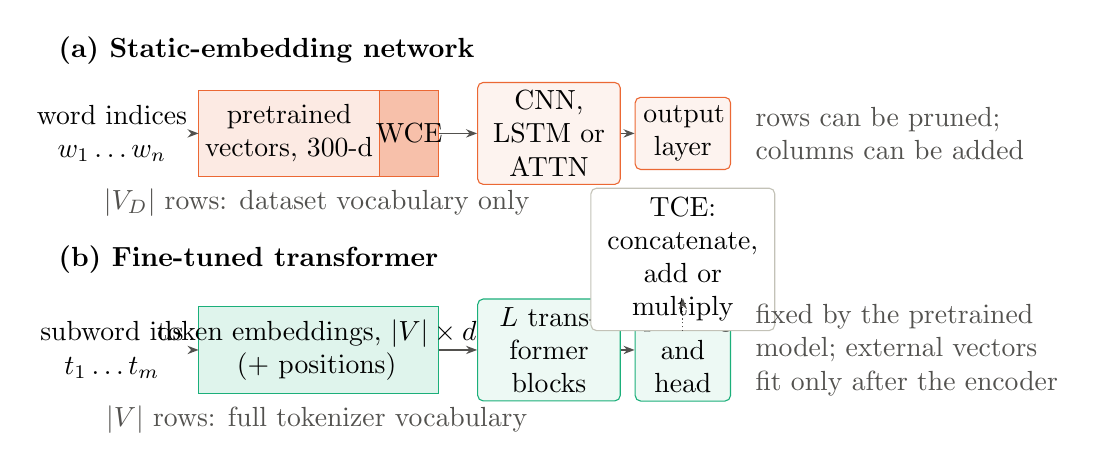
\begin{tikzpicture}[font=\figfont, >={Stealth[length=4pt]},
    blk/.style={draw=#1, fill=#1!8, rounded corners=2pt, align=center, inner sep=3pt},
    arr/.style={->, draw=inktwo, line width=0.5pt}]
  % (a) static
  \node[anchor=west, font=\figfont\bfseries] at (-0.1,1.05) {(a) Static-embedding network};
  \node[align=center] (t1) at (0.7,0) {word indices\\ $w_1 \dots w_n$};
  \fill[famST!14] (1.8,-0.55) rectangle (4.1,0.55);
  \fill[famST!42] (4.1,-0.55) rectangle (4.85,0.55);
  \draw[famST] (1.8,-0.55) rectangle (4.85,0.55);
  \draw[famST] (4.1,-0.55) -- (4.1,0.55);
  \node[align=center] at (2.95,0) {pretrained\\ vectors, 300-d};
  \node at (4.475,0) {WCE};
  \node[below, align=center, text=inktwo] at (3.3,-0.58) {$|V_D|$ rows: dataset vocabulary only};
  \node[blk=famST, text width=1.6cm] (n1) at (6.25,0) {CNN, LSTM or ATTN};
  \node[blk=famST, text width=1.0cm] (o1) at (7.95,0) {output layer};
  \draw[arr] (t1) -- (1.8,0);
  \draw[arr] (4.85,0) -- (n1);
  \draw[arr] (n1) -- (o1);
  \node[align=left, text=inktwo, anchor=west] at (8.75,0) {rows can be pruned;\\ columns can be added};
  % (b) transformer
  \node[anchor=west, font=\figfont\bfseries] at (-0.1,-1.6) {(b) Fine-tuned transformer};
  \node[align=center] (t2) at (0.7,-2.75) {subword ids\\ $t_1 \dots t_m$};
  \fill[famTR!14] (1.8,-3.3) rectangle (4.85,-2.2);
  \draw[famTR] (1.8,-3.3) rectangle (4.85,-2.2);
  \node[align=center] at (3.3,-2.75) {token embeddings, $|V| \times d$\\ (+ positions)};
  \node[below, align=center, text=inktwo] at (3.3,-3.33) {$|V|$ rows: full tokenizer vocabulary};
  \node[blk=famTR, text width=1.6cm] (n2) at (6.25,-2.75) {$L$ transformer blocks};
  \node[blk=famTR, text width=1.0cm] (o2) at (7.95,-2.75) {pooling and head};
  \draw[arr] (t2) -- (1.8,-2.75);
  \draw[arr] (4.85,-2.75) -- (n2);
  \draw[arr] (n2) -- (o2);
  \node[draw=rulegray, rounded corners=2pt, fill=white, align=center, text width=2.1cm] (tce) at (7.95,-1.6) {TCE: concatenate, add or multiply};
  \draw[->, draw=inktwo, densely dotted] (tce) -- (o2);
  \node[align=left, text=inktwo, anchor=west] at (8.75,-2.75) {fixed by the pretrained\\ model; external vectors\\ fit only after the encoder};
\end{tikzpicture}}
\caption{Where the input representation lives. (a) The static-embedding networks build their embedding layer from the corpus vocabulary and can append word-class embeddings (WCE) as extra columns. (b) A fine-tuned transformer's embedding matrix covers the model's full vocabulary, and its width is the hidden size that every pretrained layer expects, so token-class embeddings (TCE) can only be fused after the encoder.}
\label{fig:embedding}
\end{figure}

\paragraph{Token-class embeddings.} To test whether the WCE idea carries over to transformers, the transformer module computes token-class embeddings (TCEs) over each model's subword vocabulary (normalised dot product, z-scored). Concatenating TCEs at the input would change the hidden width that every pretrained layer expects, so in the logged runs they are concatenated with the pooled encoder output before the classification head and fine-tuned with the rest of the model. For BERT, DistilBERT, RoBERTa, XLNet and GPT-2, every head is run with and without TCEs on every corpus, which yields the matched pairs analysed in Section~\ref{sec:classemb}.

\subsection{Hardware and cost accounting}\label{sec:cost}

The run log records the machine for 89\% of runs (\tabref{tab:hardware}). Every logged transformer run held four GPUs under PyTorch DataParallel, on one of three machines (NVIDIA A100, RTX A6000 or RTX 6000 Ada). Every logged static-embedding run held one RTX 6000 Ada. Classical runs used CPU only: 78\% on a 64-core Linux workstation and 22\% on an Apple M3 Max laptop, including all RCV1-v2 runs.

\begin{table}[t]
\centering
\footnotesize
\caption{Hardware by module, from the run log. Share of runs: share of the module's logged runs on that machine. Software: Python 3.10, scikit-learn 1.6.1, PyTorch 2.4.1, CUDA 12.4.}
\label{tab:hardware}
\begin{tabular}{@{}lllrr@{}}
\toprule
\textbf{Module} & \textbf{Machine} & \textbf{Accelerators} & \textbf{Share of runs} & \textbf{Corpora} \\
\midrule
\inputtable{tables/tab_hardware.tex}
\bottomrule
\end{tabular}
\end{table}

We report two cost measures.
\begin{itemize}
\setlength\itemsep{1pt}
\item \emph{Training time} is the wall-clock time of model fitting as logged by each module, including all epochs up to early stopping for the neural models. It excludes data loading, preprocessing, tokenisation, the extraction of frozen embeddings for the classical module, and inference on the test set.
\item \emph{Accelerator-time} multiplies training time by the number of accelerators the run held: four GPUs for transformers, one for static-embedding networks and none for classical models. The four-fold factor measures resource occupancy, not speed-up: the runs used PyTorch's single-process DataParallel rather than distributed data parallelism, the more efficient way to train on several GPUs \cite{li2020pytorchdistributedexperiencesaccelerating}.
\end{itemize}
Because the families ran on different machines, and the transformers on three GPU types, ratios between families combine algorithmic and hardware differences. We report them as the costs a practitioner with this equipment would face, not as hardware-normalised efficiencies.

\subsection{Effectiveness measures and analysis protocol}\label{sec:protocol}

We report Macro-F1, the unweighted mean of per-class F1, and Micro-F1, F1 computed from true and false positives and false negatives pooled over classes, following \cite{moreo2021}. Macro-F1 weights rare classes as heavily as frequent ones and is the primary measure; the neural modules also use it for early stopping. Precision, recall, accuracy, Hamming loss and Jaccard index are logged but not analysed.

\paragraph{Data.} The analysis uses the run-level records of the original study: 3,725 runs (3,197 classical, 303 static-embedding, 225 transformer), each with Macro- and Micro-F1 and training time. We aggregated them per corpus and classifier into the maximum, mean, median, minimum and run count. All 784 values checked match the statistics published in \cite{worth2025layercake} to three decimals. Training time is available at full precision for 89\% of runs and rounded to the second for the rest.

\paragraph{Peak and typical scores.} A family's \emph{peak} on a corpus is its best run (ties broken by lower training time), and the cost of the peak is that run's training time. A family's \emph{typical} score is the median score of its best-by-median classifier, and its typical cost is the median training time of all its runs on the corpus. Both measures are robust to the occasional collapsed run (Section~\ref{sec:typical}). The two answer different questions. Peak asks what a family can achieve when its configuration is chosen well; typical asks what an arbitrary configuration delivers. Because the classical module explores far more configurations than the neural ones, peak comparisons favour it and typical comparisons penalise it, and we report both.

\paragraph{Statistical tests.} With eight corpora, we compare families with the exact two-sided Wilcoxon signed-rank test on per-corpus peak differences \cite{wilcoxon1945individual,demsar2006statistical}. We compare the eight classifiers with the Friedman test \cite{friedman1937use} followed by the Nemenyi post-hoc test on median scores \cite{demsar2006statistical}. For the class-embedding analyses we pair the best run with and the best run without the embeddings that share a corpus, classifier and language model (and, for static networks, the frozen-or-tuned setting), and apply the two-sided Wilcoxon test to the paired differences. Following the test-selection guidance of \cite{dror2018hitchhiker}, we use non-parametric tests, because normality of the per-corpus differences cannot be assumed with eight corpora, and we report exact $p$-values. Each configuration was run once, so differences within a single configuration cannot be tested; variation across configurations is reported instead.

\paragraph{Frontiers and tolerance.} For every corpus, the Pareto frontier is the set of runs that no other run beats on both score and training time. We also report the cheapest run within a tolerance of 1, 3 and 5 Macro-F1 points of the best, and its training time as a share of the best run's.

% ============================================================================
\section{Results}\label{sec:results}
% ============================================================================

\subsection{Peak effectiveness by family}\label{sec:peak}

\tabref{tab:peak} gives each family's peak Macro-F1 on each corpus, and \figref{fig:gaps} plots how far the best classical and static-embedding runs fall behind the best transformer. Three patterns are clear.

\begin{table}[t]
\begin{fullwidth}
\centering
\footnotesize
\setlength{\tabcolsep}{4.2pt}
\caption{Peak Macro-F1 by family on each corpus: score of the best run, the classifier (for transformers, model and head) that produced it, and its training time in seconds. The last two columns give the transformer's lead in F1 points. Micro-F1 results are in Appendix~\ref{app:micro}.}
\label{tab:peak}
\begin{tabular}{@{}lrlr rlr rlr rr@{}}
\toprule
& \multicolumn{3}{c}{\textbf{Classical ML}} & \multicolumn{3}{c}{\textbf{Static-embedding NN}} & \multicolumn{3}{c}{\textbf{Transformer}} & \multicolumn{2}{c}{\textbf{Lead (pts)}} \\
\cmidrule(lr){2-4}\cmidrule(lr){5-7}\cmidrule(lr){8-10}\cmidrule(l){11-12}
\textbf{Corpus} & F1 & clf & time & F1 & clf & time & F1 & model/head & time & vs ML & vs NN \\
\midrule
\inputtable{tables/tab_peak_macro.tex}
\bottomrule
\end{tabular}
\end{fullwidth}
\end{table}

\begin{figure}[t]
\centering
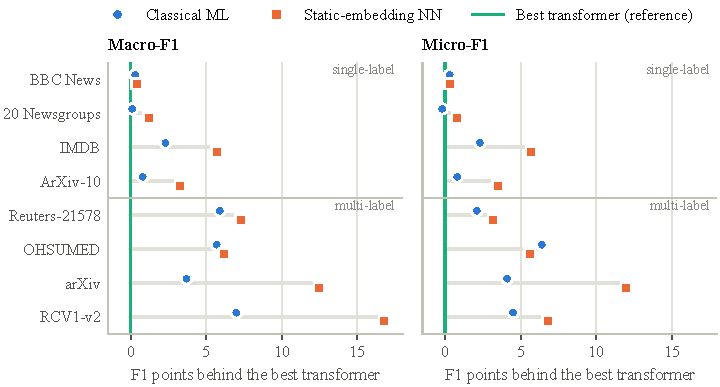
\includegraphics[width=\textwidth]{pictures/fig_peak_gaps.pdf}
\caption{Distance of the best classical (circles) and best static-embedding (squares) run from the best fine-tuned transformer run on each corpus, in F1 points. Single-label corpora are above the rule, multi-label corpora below. Values are in \tabref{tab:peak} and Appendix~\ref{app:micro}.}
\label{fig:gaps}
\end{figure}

\begin{table}[t]
\centering
\footnotesize
\caption{Family comparisons across the eight corpora. Peak lead: mean difference in peak F1 (points), with range. W/T/L: corpora won, tied and lost by the first family. $p$: exact two-sided Wilcoxon signed-rank test on the per-corpus peak differences (ties dropped). Typical lead: mean difference between the families' typical (median) scores.}
\label{tab:tests}
\begin{tabular}{@{}lrcccr@{}}
\toprule
& \textbf{Peak lead} & \textbf{Range} & \textbf{W/T/L} & \textbf{$p$} & \textbf{Typical lead} \\
\midrule
\inputtable{tables/tab_tests.tex}
\bottomrule
\end{tabular}
\end{table}

First, fine-tuned transformers have the highest peak Macro-F1 on all eight corpora. Their mean peak is 0.808, against 0.776 for the classical family and 0.741 for static-embedding networks. The advantage over each of the other families is consistent in sign ($p = 0.0078$, the smallest attainable $p$ with eight corpora; \tabref{tab:tests}) but modest in size: 3.2 points over the classical family and 6.7 points over the static networks on average. For Micro-F1 the leads shrink to 2.5 and 4.7 points, and on 20~Newsgroups the best classical run has the higher Micro-F1. The transformer peak comes from DeepSeek-R1-Distill on four corpora, from RoBERTa on three and from XLNet on one; Section~\ref{sec:lms} asks what the larger models cost.

Second, the best classical run beats the best static-embedding run on all eight corpora for Macro-F1 (mean $+3.5$ points, $p = 0.0078$) and wins six of eight for Micro-F1, with one tie and one loss. This reverses the ordering usually assumed between linear models and neural networks over word vectors. It depends, however, on which features the linear model receives. The winning classical configuration on six corpora concatenates sparse features with mean-pooled embeddings from a frozen transformer, most often Llama-3.2-1B (Appendix~\ref{app:configs}). Only on OHSUMED (TF-IDF alone) and Reuters-21578 (TF-IDF with pooled fastText vectors) does the best classical configuration use no transformer at all.

Third, the transformer premium depends on the task type. On the four single-label corpora the best classical run trails the best transformer by 0.1--2.3 Macro-F1 points (mean 0.9). On the four multi-label corpora, which have 23--115 classes and long-tailed label distributions, it trails by 3.7--7.0 points (mean 5.6). With four corpora per group the separation is suggestive rather than conclusive (exact Mann--Whitney $p = 0.029$ for Macro-F1 and $0.057$ for Micro-F1). Multi-label status is also confounded with the number of classes and with corpus size. The pattern is nevertheless consistent with Macro-F1 rewarding performance on rare classes, where a fine-tuned encoder's contextual features help most.

\subsection{Typical configurations and robustness}\label{sec:typical}

Peak scores reward exhaustive search, and the classical module searches far more broadly than the neural ones. Typical scores reverse part of the picture (\tabref{tab:tests}, last column). The median configuration of the best transformer classifier leads the median classical configuration by 7.8 Macro-F1 points, more than twice the peak lead, while the median static-embedding network edges out the median classical configuration by 1.2 points. In other words, classical models reach transformer-like scores only when their features are chosen well; many of their configurations, including all naive Bayes runs, are much weaker. Transformers are comparatively insensitive to the choice of model and head.

\figref{fig:cd} ranks all eight classifiers by median score on each corpus. The Friedman test rejects equal performance for both Macro-F1 ($\chi^2_7 = 29.9$, $p = 1.0\times10^{-4}$) and Micro-F1 ($\chi^2_7 = 31.9$, $p = 4.3\times10^{-5}$). With eight corpora, however, the Nemenyi critical difference is 3.71 ranks, so only the largest gaps are resolved:
\begin{itemize}
\setlength\itemsep{1pt}
\item Macro-F1: HF-CNN ranks significantly above the linear SVM and NB, and HF-SC above NB.
\item Micro-F1: both transformer heads rank above the SVM and NB.
\end{itemize}
No difference between the transformer heads and the static networks, or between the static networks and LR, is significant at this sample size.

\begin{figure}[t]
\centering
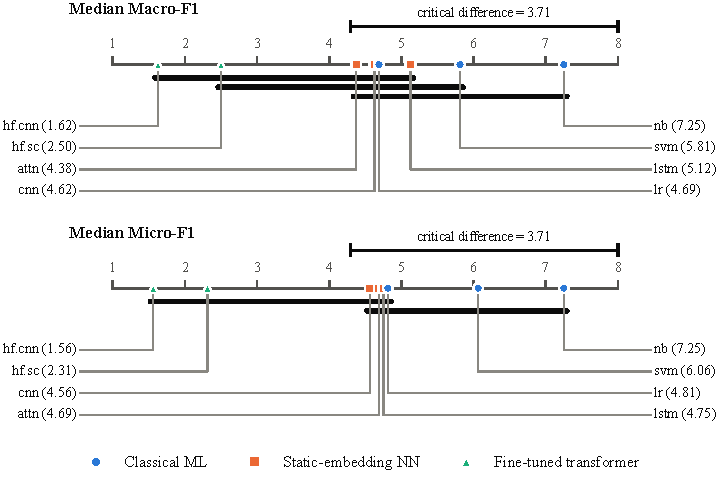
\includegraphics[width=\textwidth]{pictures/fig_cd.pdf}
\caption{Critical-difference diagrams: average rank of each classifier by median score across the eight corpora (1 = best). Classifiers joined by a bar are not significantly different (Nemenyi, $\alpha = 0.05$, critical difference 3.71). Marker shape and colour give the family.}
\label{fig:cd}
\end{figure}

Medians also guard against a failure mode visible in the run log. Of the 528 neural runs, nine have a Macro-F1 below 0.35:
\begin{itemize}
\setlength\itemsep{1pt}
\item On arXiv, three HF-SC runs (BERT, and DistilBERT with and without TCEs) score 0.000, and five LSTM runs score between 0.000 and 0.348.
\item On IMDB, one Llama-3.2-1B HF-CNN run predicts a single class: Macro-F1 0.333, the score of a constant classifier on a balanced binary task.
\end{itemize}
These runs pull the HF-SC mean on arXiv to 0.547 against a median of 0.681. Averaged results, as reported in \cite{worth2025layercake}, are sensitive to such runs; peak and median results are not.

\subsection{What the last points cost}\label{sec:costresults}

\tabref{tab:cost} sets the transformer's lead on each corpus against the typical training time of each family. A typical transformer run trains 25--45 times longer than a typical static-embedding run (geometric mean 32$\times$). Counting the four GPUs it held, that is 127 times the accelerator-time. It trains 24--133 times longer than a typical classical run (geometric mean 75$\times$). The winning runs are costlier still, because the transformer peak is often reached by one of the two large models: in wall-clock time, the best transformer run took 19--146 times as long as the best static-embedding run (geometric mean 61$\times$).

\begin{table}[t]
\centering
\footnotesize
\setlength{\tabcolsep}{4.5pt}
\caption{The transformer's peak Macro-F1 lead (points) and the median training time (seconds) of each family's runs on each corpus, with the ratio of the transformer median to the static-embedding and classical medians. Multiply the first ratio by four for accelerator-time.}
\label{tab:cost}
\begin{tabular}{@{}lrrrrrrr@{}}
\toprule
& \multicolumn{2}{c}{\textbf{Lead (pts)}} & \multicolumn{3}{c}{\textbf{Median training time (s)}} & \multicolumn{2}{c}{\textbf{Transformer time}} \\
\cmidrule(lr){2-3}\cmidrule(lr){4-6}\cmidrule(l){7-8}
\textbf{Corpus} & \textbf{vs ML} & \textbf{vs NN} & \textbf{ML} & \textbf{NN} & \textbf{Transf.} & \textbf{/ NN} & \textbf{/ ML} \\
\midrule
\inputtable{tables/tab_cost.tex}
\bottomrule
\end{tabular}
\end{table}

Ratios between families hide the runs in between. \figref{fig:pareto} plots every run against its training time and draws the Pareto frontier. On every corpus the frontier ends at a transformer run, so a transformer is always the most accurate choice. Below that point, classical runs dominate. Across the eight corpora, 96 runs lie on a Macro-F1 frontier: 71 classical and 25 transformer. No static-embedding run does; for Micro-F1, four do, on OHSUMED and RCV1-v2. The frontiers have two shapes:
\begin{itemize}
\setlength\itemsep{1pt}
\item On the single-label corpora they flatten early: the best classical run comes within 0.1--2.3 points of the best transformer run at 12 to 239 times less training time.
\item On Reuters-21578, OHSUMED, arXiv and RCV1-v2 they end in a tall final step, where transformer runs add several points at the far right of the time axis.
\end{itemize}

\begin{figure}[t]
\centering
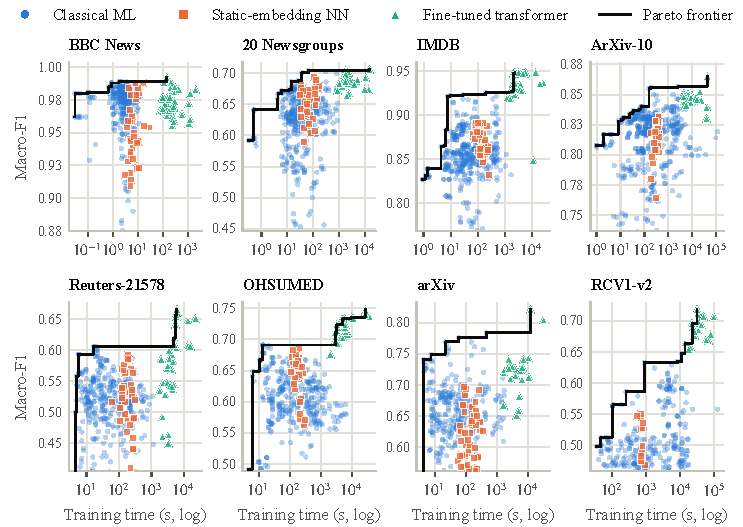
\includegraphics[width=\textwidth]{pictures/fig_pareto.pdf}
\caption{Macro-F1 against training time (log scale) for every run on each corpus; the line is the Pareto frontier. Classical runs are drawn small and translucent because there are several hundred per corpus. Vertical axes differ between panels and are cropped to the upper part of each corpus's range.}
\label{fig:pareto}
\end{figure}

\tabref{tab:tolerance} turns the frontier into a decision rule: for a given tolerance, what is the cheapest run and what share of the best run's training time does it need?
\begin{itemize}
\setlength\itemsep{1pt}
\item \textbf{Single-label corpora.} A tolerance of one point is enough to replace the transformer on BBC News, 20~Newsgroups and ArXiv-10 with a linear model that trains in 0.23--0.47\% of the time. On IMDB a three-point tolerance does the same at 0.32\%.
\item \textbf{Multi-label corpora.} No tolerance up to three points admits anything but a transformer. However, a base-size encoder often comes close to the large model that holds the peak: on OHSUMED, RoBERTa comes within 2.4 points at 12\% of DeepSeek's training time. At five points a classical SVM appears on arXiv at 0.48\% of the time, but on Reuters-21578, OHSUMED and RCV1-v2 even a five-point tolerance still requires a transformer.
\end{itemize}

\begin{table}[t]
\begin{fullwidth}
\centering
\scriptsize
\setlength{\tabcolsep}{4pt}
\caption{Cheapest run within 1, 3 and 5 Macro-F1 points of the best run on each corpus: model, its Macro-F1, and its training time as a share of the best run's (--- : only the best run qualifies). Classical entries give the classifier and the language model whose embeddings, projections or tokenizer the features use; their extraction time is not included.}
\label{tab:tolerance}
\begin{tabularx}{\linewidth}{@{}l>{\raggedright}p{1.85cm}r>{\raggedright}X>{\raggedright}X>{\raggedright\arraybackslash}X@{}}
\toprule
\textbf{Corpus} & \textbf{Best run} & \textbf{Time (s)} & \textbf{Within 1 pt} & \textbf{Within 3 pts} & \textbf{Within 5 pts} \\
\midrule
\inputtable{tables/tab_tolerance.tex}
\bottomrule
\end{tabularx}
\end{fullwidth}
\end{table}

These comparisons understate the cost of classical runs that use transformer features, because extracting those features requires one forward pass of the frozen transformer over the training and test documents, which is not timed. That pass is cheaper than fine-tuning, since it involves no backward pass and a single epoch, but it is not free; on RCV1-v2, whose test set has 781,265 documents, it is substantial. The comparisons also understate the cost of transformers in deployment, because inference on new documents is excluded for every family and is most expensive for transformers. The decision rule in \tabref{tab:tolerance} is therefore conservative for single-label tasks with a modest test volume, which is where it recommends the cheaper models.

\subsection{Which transformer?}\label{sec:lms}

Within the transformer family, model size and training time vary by an order of magnitude. \tabref{tab:lmresults} and \figref{fig:lms} compare the seven models by their best Macro-F1 on each corpus and by their median training time relative to BERT on the same corpus. The models differ ($\chi^2_6 = 18.9$, $p = 0.004$, Friedman), but not in proportion to their cost:
\begin{itemize}
\setlength\itemsep{1pt}
\item \textbf{DeepSeek-R1-Distill} has the best average rank (2.38) and wins four corpora, but takes a median 6.6 times as long as BERT.
\item \textbf{RoBERTa} wins three corpora at 1.1 times BERT's time, and \textbf{XLNet} two at 2.2 times (the two tie on IMDB).
\item \textbf{Llama-3.2-1B} ranks sixth of seven, on average 4.7 points behind the best model, at 5.1 times BERT's time.
\end{itemize}

\begin{table}[t]
\centering
\footnotesize
\caption{Fine-tuned transformer models across the eight corpora (Macro-F1; best run per model and corpus over both heads, with and without TCEs). Rank: average rank (1 = best). Wins: corpora on which the model is best. Behind: mean and maximum points behind the best model on the corpus. Time: median training time relative to BERT on the same corpus.}
\label{tab:lmresults}
\begin{tabular}{@{}lrrrrr@{}}
\toprule
\textbf{Model} & \textbf{Rank} & \textbf{Wins} & \textbf{Behind (mean)} & \textbf{Behind (max)} & \textbf{Time} \\
\midrule
\inputtable{tables/tab_lms.tex}
\bottomrule
\end{tabular}
\end{table}

\begin{figure}[t]
\centering
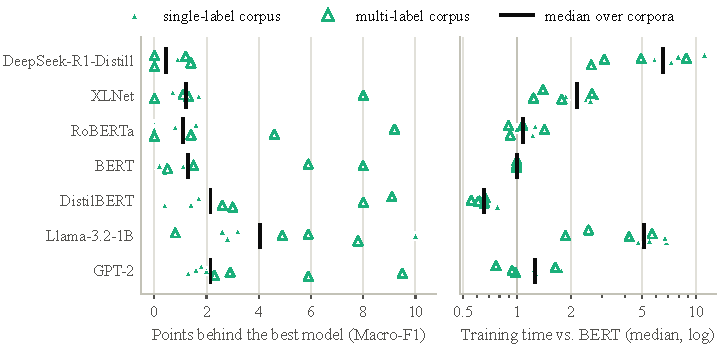
\includegraphics[width=\textwidth]{pictures/fig_lms.pdf}
\caption{Fine-tuned transformer models: Macro-F1 points behind the best model on each corpus (left) and median training time relative to BERT (right, log scale). Each marker is one corpus; bars are medians. Filled markers are single-label corpora, open markers multi-label.}
\label{fig:lms}
\end{figure}

Comparing, on each corpus, the better of the two large decoders with the best base-size encoder (BERT, RoBERTa, DistilBERT or XLNet):
\begin{itemize}
\setlength\itemsep{1pt}
\item the large models gain 8.0 points on arXiv, 1.3 on ArXiv-10 and OHSUMED, and 0.2 on 20~Newsgroups;
\item they lose 0.9--1.4 points on the other four corpora (median change $-0.4$, mean $+0.8$);
\item they need 2.3--7.2 times the training time (geometric mean 4.9).
\end{itemize}
The one clear win, arXiv, is a corpus of long, technical abstracts on which DeepSeek-R1-Distill, whose base model was trained for mathematical reasoning, leads every other model by at least 7.8 points. Elsewhere, the extra parameters buy little. DistilBERT trains in two-thirds of BERT's time and trails the best base encoder by a median of 1.4 points, though by 8.0 on Reuters-21578, the corpus with the most classes.

\subsection{Representation choices for classical models}\label{sec:forms}

Within the classical family, which representation pays? \figref{fig:solo} compares pooled embeddings alone (\emph{solo}, 300--2,048 dimensions) with the best representation form on each corpus. On six corpora, pooled embeddings come within 0.1--2.1 Macro-F1 points of the best form, usually \emph{cat-doc} (sparse features concatenated with pooled embeddings). On ArXiv-10, IMDB and RCV1-v2 the extra 0.1--1.5 points cost 8--14 times the median training time. The exceptions are OHSUMED, where the best form is TF-IDF alone, 7.5 points ahead of pooled embeddings and faster, and Reuters-21578, where \emph{cat-doc} leads by 3.9 points.

\begin{figure}[t]
\centering
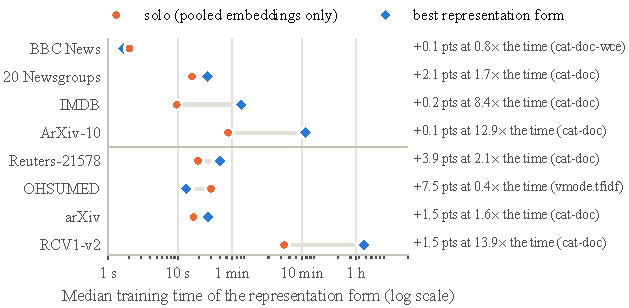
\includegraphics[width=\textwidth]{pictures/fig_solo.pdf}
\caption{Pooled embeddings alone (\emph{solo}) against the best classical representation form on each corpus (Macro-F1 of the best run of each form; median training time of each form's runs).}
\label{fig:solo}
\end{figure}

\subsection{Class embeddings: static networks yes, transformers no}\label{sec:classemb}

\tabref{tab:classemb} and \figref{fig:classemb} summarise every matched comparison of a model with and without class embeddings.

\begin{table}[t]
\begin{fullwidth}
\centering
\footnotesize
\setlength{\tabcolsep}{5pt}
\caption{Effect of class embeddings on matched runs (best run with vs.\ without, same corpus, classifier and language model). Median change in F1 points, number of pairs that improved/worsened, two-sided Wilcoxon $p$, and median training-time multiple. For the classical module, rows give the representation form the WCEs are added to.}
\label{tab:classemb}
\begin{tabular}{@{}lr rrr rrr r@{}}
\toprule
& & \multicolumn{3}{c}{\textbf{Macro-F1}} & \multicolumn{3}{c}{\textbf{Micro-F1}} & \\
\cmidrule(lr){3-5}\cmidrule(lr){6-8}
\textbf{Setting} & \textbf{Pairs} & \textbf{Median} & \textbf{Up/down} & \textbf{$p$} & \textbf{Median} & \textbf{Up/down} & \textbf{$p$} & \textbf{Time} \\
\midrule
\inputtable{tables/tab_classemb.tex}
\bottomrule
\end{tabular}
\end{fullwidth}
\end{table}

\begin{figure}[t]
\centering
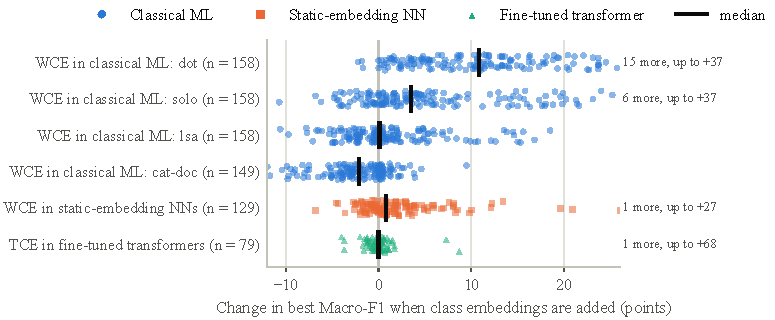
\includegraphics[width=\textwidth]{pictures/fig_classemb.pdf}
\caption{Change in best Macro-F1 when class embeddings are added, for every matched pair. Bars are medians. Pairs beyond the right edge are counted in the margin; the single TCE outlier (+68) is a pair in which the run without TCEs collapsed.}
\label{fig:classemb}
\end{figure}

\paragraph{Static-embedding networks.} WCEs help. Across 129 pairs (same corpus, network, word model and frozen-or-tuned setting), they raise Macro-F1 by a median of 0.8 points (mean 2.3) and improve 80 pairs against 45 ($p = 1.5\times10^{-6}$), at no extra training time. The gains are largest on arXiv (mean $+8.6$) and Reuters-21578 ($+4.8$), the corpora with the most classes outside RCV1-v2, and slightly negative on ArXiv-10, IMDB and RCV1-v2. This is consistent with the gains reported by \cite{moreo2021}, here across eight corpora.

\paragraph{Classical models.} The effect of WCEs depends on what they are added to. They transform the weakest dense representation: projecting TF-IDF through the WCE-extended space (\emph{dot-wce}) beats the plain projection in 153 of 158 pairs, by a median of 10.9 points. They also lift pooled embeddings (\emph{solo}, median $+3.5$, 118 of 158 pairs). They leave LSA unchanged ($+0.1$, $p = 0.21$), and they \emph{lower} \emph{cat-doc} in 102 of 149 pairs (median $-2.1$), where the sparse vector already carries the lexical evidence the WCEs summarise. They also cost up to 2.6 times the training time. WCEs thus act as a supplement for weak representations rather than an improvement to strong ones.

\paragraph{Fine-tuned transformers.} TCEs have no effect. Across 79 pairs (same corpus, model, vocabulary and head), the median change in Macro-F1 is 0.0 points: 39 pairs improve, 35 worsen and 5 tie ($p = 0.66$). The mean change ($+0.9$) is carried entirely by one arXiv pair in which the run without TCEs collapsed. Excluding the two pairs with a collapsed run, the mean change is 0.00 points ($p = 0.52$). Micro-F1 behaves the same way. This corrects the earlier report that TCEs consistently \emph{degraded} transformer performance \cite{worth2025layercake}: in the logged runs they neither help nor hurt. A plausible explanation is that fine-tuning already shapes the encoder's representation around the label set, so token--class statistics fused after the encoder add nothing the head does not already see. Injecting class information earlier, for instance into intermediate layers through a learned projection, remains untested.

% ============================================================================
\section{Discussion}\label{sec:discussion}
% ============================================================================

\subsection{Choosing a classifier}

The results support a simple procedure.
\begin{enumerate}
\setlength\itemsep{1pt}
\item Start with a linear model over TF-IDF features concatenated with mean-pooled embeddings from a frozen transformer; logistic regression and a linear SVM are both strong. For a single-label task with a handful of classes, this configuration is likely to come within one to three points of a fine-tuned transformer at well under one percent of its training time.
\item For a multi-label task with many classes, especially when Macro-F1 (performance on rare classes) matters, expect fine-tuning to add four to seven points.
\item If you fine-tune, start with a base-size encoder such as RoBERTa or BERT. Here the billion-parameter-scale decoders cost about five times as much for no consistent gain; the exception was the technical arXiv corpus.
\item Do not expect token-class embeddings to help a fine-tuned transformer. They remain worth adding to static-embedding networks and to weak pooled features.
\end{enumerate}
Static-embedding neural networks occupy an awkward middle: on these corpora they were never more accurate than the best linear configuration and never on the Macro-F1 cost frontier.

This procedure also fits how such systems are run. A classifier that is retrained whenever labels drift or categories change pays its training cost repeatedly, so a typical training-time ratio of 30 to 75 compounds over the life of the system. Where the cheaper model is within the tolerance the application can bear, \tabref{tab:tolerance} identifies it.

\subsection{Why frozen embeddings and linear models do so well}

Contextual token representations are highly anisotropic \cite{ethayarajh2019contextual}, which carries over to their mean-pooled averages. Sentence-embedding work also shows that naively pooling a model trained for a different objective gives weak sentence vectors \cite{reimers2019sentence}. Yet for topic and sentiment classes that are separable by vocabulary and broad semantics, a linear model over such features, alongside the sparse TF-IDF vector that keeps exact lexical evidence, is enough. Pooled features and sparse features are complementary: the best classical configuration on six corpora uses both. What fine-tuning adds is a representation shaped by the label set. That matters most when there are many classes, some of them rare and distinguished by subtle contextual cues, which is the multi-label regime in our data.

\subsection{Limitations}

\begin{itemize}
\setlength\itemsep{1pt}
\item \textbf{Heterogeneous hardware.} The families ran on different machines and the transformers on three GPU types (\tabref{tab:hardware}). The ratios are therefore costs on this equipment, not hardware-normalised efficiencies.
\item \textbf{What is timed.} Training time excludes feature extraction, including the frozen transformer pass that the best classical configurations depend on, and excludes inference for all families.
\item \textbf{Unequal search budgets.} The classical module explores 171--244 configurations per corpus for each of LR and the SVM, the neural modules 4--25 per classifier. This favours the classical family at peak and penalises it in typical comparisons, which is why we report both.
\item \textbf{Single runs.} Each configuration was run once. Peak scores are therefore maxima over configurations, not means over seeds, and on the closest comparisons (BBC News, 20~Newsgroups) differences of a few tenths of a point are within the range that seed variation could produce.
\item \textbf{Defaults and scale.} Classical models used default hyperparameters; tuning them would likely help them further. The transformers are at most 1.5B parameters, fine-tuned in full with DataParallel. Parameter-efficient fine-tuning, distributed data parallelism and larger models would change both sides of the trade-off.
\item \textbf{Time precision.} For 11\% of runs the training time is available only rounded to the second, which matters only for the fastest classical runs.
\end{itemize}

% ============================================================================
\section{Conclusion}\label{sec:conclusion}
% ============================================================================

How much accuracy does fine-tuning a transformer buy for text classification, and at what cost? Across 3,725 runs on eight corpora, the answer is: on every corpus some, but on average little relative to a well-chosen linear model (3.2 Macro-F1 points), at a typical training-time multiple of 75. The average hides a clear split. On single-label tasks, a linear model over frozen, pooled transformer features comes within 0.5--2.7 points at well under one percent of the best run's training time. On multi-label, many-class tasks, the transformer's lead of four to seven points has no linear substitute, though a base-size encoder is usually enough. Static-embedding networks were dominated throughout; billion-parameter-scale decoders rarely repaid their cost; and token-class embeddings, unlike their word-level counterparts in static networks, had no effect on fine-tuned transformers. These differences become visible only by reporting peak and typical scores, paired tests, accelerator-time, Pareto frontiers and tolerance tables, rather than averages over unequal numbers of configurations. We recommend the same protocol for other comparisons of model families.

Two extensions would sharpen these conclusions. The first is to time feature extraction and inference, so that the frozen-feature configurations and deployed transformers are costed in full. The second is to add the efficient alternatives that have matured since these runs: parameter-efficient fine-tuning \cite{hu2021loralowrankadaptationlarge,dettmers2023qloraefficientfinetuningquantized}, modern efficient encoders such as ModernBERT \cite{warner2024modernbert}, few-shot sentence-embedding classifiers such as SetFit \cite{tunstall2022setfit}, and prompted LLMs \cite{edwards2024language}. Layer Cake and the analysis scripts released with this article are designed to make each of these a configuration change rather than a new study.

\componenthead{Data and Code Availability}
The Layer Cake framework is available at \url{https://github.com/pworth1971/layer-cake}. The run-level results of the original study, the summary tables of the earlier paper, and the scripts that produce every table and figure in this article (\texttt{extract\_tables.py}, \texttt{extract\_runs.py}, \texttt{analyze.py}, \texttt{tables.py}, \texttt{figures.py}) are in the \texttt{paper/scirp/V7} directory of the same repository.

\componenthead{Acknowledgements}
In preparing this revision the author used Claude Code (Anthropic), an AI assistant for software and writing tasks, through its Visual Studio Code extension, with the Claude Opus 5.5 model (\texttt{claude-opus-5-5}), on 23 October 2026. The assistant was used to:
\begin{itemize}
\item redraft and restructure the manuscript from the earlier version \cite{worth2025layercake};
\item write the analysis scripts released with this article, re-analyse the published run-level results with them, and check that they reproduce every summary statistic reported in \cite{worth2025layercake};
\item check each reference against Crossref, arXiv, the ACL Anthology and publisher records, and correct the bibliography;
\item regenerate the figures and tables, and typeset the manuscript in the journal template.
\end{itemize}
No new experiments were run, and the assistant neither generated nor altered any experimental result. The author reviewed and edited all AI-assisted material and takes full responsibility for the content of this article.

\componenthead{Author Contributions}
P.J.W. is the sole author of this work and is responsible for its conceptualization, methodology, software, investigation (all experiments), formal analysis, data curation, visualization, and writing (original draft, review and editing).

\componenthead{Conflicts of Interest}
The author declares no conflicts of interest regarding the publication of this paper.

\bibliographystyle{scirp}
\bibliography{lc_v7_refs}

% ============================================================================
\appendix
\renewcommand{\thesection}{\Alph{section}}
\setcounter{table}{0}
\renewcommand{\thetable}{A\arabic{table}}
\section{Supplementary Results}
% ============================================================================

\subsection{Peak Micro-F1 by family}\label{app:micro}

\begin{table}[H]
\begin{fullwidth}
\centering
\footnotesize
\setlength{\tabcolsep}{4.2pt}
\caption{Peak Micro-F1 by family (as \tabref{tab:peak}).}
\label{tab:peakmicro}
\begin{tabular}{@{}lrlr rlr rlr rr@{}}
\toprule
& \multicolumn{3}{c}{\textbf{Classical ML}} & \multicolumn{3}{c}{\textbf{Static-embedding NN}} & \multicolumn{3}{c}{\textbf{Transformer}} & \multicolumn{2}{c}{\textbf{Lead (pts)}} \\
\cmidrule(lr){2-4}\cmidrule(lr){5-7}\cmidrule(lr){8-10}\cmidrule(l){11-12}
\textbf{Corpus} & F1 & clf & time & F1 & clf & time & F1 & model/head & time & vs ML & vs NN \\
\midrule
\inputtable{tables/tab_peak_micro.tex}
\bottomrule
\end{tabular}
\end{fullwidth}
\end{table}

\subsection{Best classical configurations}\label{app:configs}

\begin{table}[H]
\centering
\footnotesize
\caption{Feature set of the best classical run on each corpus (notation of Section~\ref{sec:representations}; a model name denotes its mean-pooled frozen embeddings).}
\label{tab:configs}
\begin{tabular}{@{}llp{6.2cm}r@{}}
\toprule
\textbf{Corpus} & \textbf{Clf} & \textbf{Features} & \textbf{F1} \\
\midrule
\multicolumn{4}{@{}l}{\textit{Macro-F1}} \\
\inputtable{tables/tab_mlconfigs_macro.tex}
\midrule
\multicolumn{4}{@{}l}{\textit{Micro-F1}} \\
\inputtable{tables/tab_mlconfigs_micro.tex}
\bottomrule
\end{tabular}
\end{table}

\subsection{Validation splits}\label{app:splits}

\begin{table}[H]
\centering
\footnotesize
\caption{Training and validation sizes in the neural modules. Test sets are those of \tabref{tab:datasets}.}
\label{tab:splits}
\begin{tabular}{@{}lrrrr@{}}
\toprule
& \multicolumn{2}{c}{\textbf{Static-embedding NN}} & \multicolumn{2}{c}{\textbf{Transformer}} \\
\cmidrule(lr){2-3}\cmidrule(l){4-5}
\textbf{Corpus} & \textbf{Train} & \textbf{Validation} & \textbf{Train} & \textbf{Validation} \\
\midrule
\inputtable{tables/tab_splits.tex}
\bottomrule
\end{tabular}
\end{table}

\subsection{Per-classifier results}\label{app:perclf}

\tabsref{tab:appmacro}{tab:appmicro} give, for each corpus and classifier, the maximum, median, mean and minimum score across runs, the number of runs and the median training time. Mean and run count match the corresponding statistics of \cite{worth2025layercake}.

\begin{table}[p]
\centering
\scriptsize
\caption{Macro-F1 by corpus and classifier.}
\label{tab:appmacro}
\begin{tabular}{@{}llrrrrrr@{}}
\toprule
\textbf{Corpus} & \textbf{Clf} & \textbf{Max} & \textbf{Median} & \textbf{Mean} & \textbf{Min} & \textbf{Runs} & \textbf{Time (s)} \\
\midrule
\inputtable{tables/tab_appendix_macro.tex}
\bottomrule
\end{tabular}
\end{table}

\begin{table}[p]
\centering
\scriptsize
\caption{Micro-F1 by corpus and classifier.}
\label{tab:appmicro}
\begin{tabular}{@{}llrrrrrr@{}}
\toprule
\textbf{Corpus} & \textbf{Clf} & \textbf{Max} & \textbf{Median} & \textbf{Mean} & \textbf{Min} & \textbf{Runs} & \textbf{Time (s)} \\
\midrule
\inputtable{tables/tab_appendix_micro.tex}
\bottomrule
\end{tabular}
\end{table}

\end{document}
